%%%%%%%% COMP1801 EXAMPLE LATEX FILE %%%%%%%%%%%%%%%%%
% This template and document is based on \href{https://media.icml.cc/Conferences/ICML2021/Styles/icml2021\_style.zip}{ICML 2021 LaTeX style file} (\url{https://media.icml.cc/Conferences/ICML2021/Styles/icml2021\_style.zip})
% Modified from a template file originally constructed by Atsushi Suzuki and Jing Wang
% Copyright (the body text): Peter Soar, 2022-2024.

%%%%%%%%%%%%%%%%%%%%%%%%%%%%%%%%%%%%%%%%%%%%%%%%%%%%%%%%%%%%%%%%%%%%%

% Welcome to latex! This may all seem a bit confusing if you have only made documents using MS word before, but as computing MSc students hopefully a bit of source code won't worry you too much.

% Immediately below here are the packages that our document is using, along with other header material that tells the document how to behave when compiled. While for your coursework you shouldn't have to alter any of this  header information, if you want to start using Latex for your own documents you will certainly want to learn about what kind of packages are available, as they can certainly save a lot of time to get you document looking exactly how you want!

%%%%%%%%%%%%%%%%%%%%%%%%%%%%%%%%%%%%%%%%%%%%%%%%%%%%%%%%%%%%%%%%%%%%%%%%%
% Header Information and Packages
% Scroll down to the main document
%%%%%%%%%%%%%%%%%%%%%%%%%%%%%%%%%%%%%%%%%%%%%%%%%%%%%%%%%%%%%%%%%%%%%%%%%

\documentclass{article}
% Recommended, but optional, packages for figures and better typesetting:
%\usepackage{microtype}
\usepackage{graphicx}
%\usepackage{subfigure}
\usepackage{subcaption}
\usepackage{booktabs} % for professional tables

\usepackage[style=authoryear,backend=biber]{biblatex}
\addbibresource{T0-Exercise.bib}% Syntax for version >= 1.2

\usepackage{amsmath}
\usepackage{amsfonts}
\usepackage{amsthm}
\usepackage{physics}
\usepackage{fancyvrb}
\usepackage{caption}
% hyperref makes hyperlinks in the resulting PDF.
\usepackage{xurl}
\usepackage{hyperref}

% Attempt to make hyperref and algorithmic work together better:
\newcommand{\theHalgorithm}{\arabic{algorithm}}

\usepackage{accessibility}

\usepackage{Coursework}

\begin{document}
%%%%%%%%%%%%%%%%%%%%%%%%%%%%%%%%%%%%%%%%%%%%%%%%%%%%%%%%%%%%%%%%%%%%%%%%%
% Main document begins
% From here onward contains the actual document contents that will be seen in the compiled PDF
%%%%%%%%%%%%%%%%%%%%%%%%%%%%%%%%%%%%%%%%%%%%%%%%%%%%%%%%%%%%%%%%%%%%%%%%%

\cwtitle{Latex Introduction Exercise}

\section{Introduction}

This document\footnote{This template and document is based on \href{https://media.icml.cc/Conferences/ICML2021/Styles/icml2021\_style.zip}{ICML 2021 LaTeX style file} (\url{https://media.icml.cc/Conferences/ICML2021/Styles/icml2021\_style.zip})} has been put together to introduce you to \LaTeX, give you an idea how to layout a document and show you how to use the main functionality you are likely to need. For the coursework you will be given preexisting \LaTeX template like this, where all you should need to change is the body text to represent your work.

\section{How to use \LaTeX?}
\LaTeX is a word processing application now which has been increasing with popularity over recent years. Especially in some academic circles it has begun to be regarded as a de-facto standard word processing application.
The following is quick guide for the anatomy of a \LaTeX document.
\begin{itemize}
    \item \verb|T0-Exercise.tex| is the file you are inside now which contains all the information you want to appear in your document, including the title, the main body text, etc
    \item The \verb|.sty| files controls all of the default page layout and functions used by your \LaTeX file. If you get into using \LaTeX you may want to start altering these, but for the purposes of this module you can (and should!) leave them as they are.
    \item \verb|T0-Exercise.bib| file manages and references you want to use in your document, which you can copy into this file in a \verb|BibTex| format from google scholar or elsewhere. However, for this coursework module I will \textbf{not} require you to use any references in the coursework report, but you are encouraged to include them if you feel it is appropriate.
    \item You can see a folder called 'Images' which contains some \verb|.png| files I want to load into the document. Images you use have to be uploaded into the file system on the left, but they don't need to be inside a folder (I just think it makes things much neater when you start getting lots of images).
    \item Some basic \LaTeX commands lets you make text \textbf{bold}, \emph{italic} and \textunderscore{underlined}.
    \item You can insert a line break using \verb|\\| or by leaving a blank line in the source code.
    \item The configuration is described before \verb|\begin{document}| command, and the body text (anything you want to appear in your document) should be described between \verb|\begin{document}| and \verb|\end{document}| commands. 
    \item You can change the title by editing the operands of \verb|\cwtitle| commands. You can find this before \verb|\begin{document}|.
    \item You can use \verb|\section|, \verb|\subsection|, \verb|\subsubsection| to create a section, subsection, and subsubsection headings in the body text. 
    Partitioning a text using these commands may improve the readability.
    \item You can use numerous commands to write mathematical symbols, lists, images, tables, etc. A cheat sheet of many of the key ones can be found in this \href{https://v1.overleaf.com/latex/templates/a-quick-guide-to-latex/fghqpfgnxggz.pdf}{Quick guide to \LaTeX} which should help you do most things you would want to do.
    \item I will show you how to add tables and figures to a \LaTeX document below. However, \LaTeX will try and put decide for you the best way to insert these images into your final PDF to make the best page layout. While this is usually good, sometimes you will want to override \LaTeX at the expense of good page layout. You can find the positioning parameters  \href{https://www.overleaf.com/learn/latex/Positioning_of_Figures}{here}
\end{itemize}


\section{Comments}
You've probably noticed by now, but like in most coding languages, \LaTeX allows you to make comments in the source code which have no impact on how the code runs (or in this case, the PDF compiled). You can do this using the \verb|%| symbol at the start of a line in the source code.
%This can be helpful for writing any reminders or points that you need to remind yourself of while writing, but which shouldn't appear in the final document. 


\section{lists}
While I have used one above, it is also worth noting that you can make bullet point lists in \LaTeX using \verb|itemize| like so:
\begin{itemize}
    \item Point 1
    \item Point 2
    \item Point 3
\end{itemize}

and you can get numbered lists using \verb|enumerate|:
\begin{enumerate}
  \item Numbers are generated automatically.
  \item Every new enumerate will start at 1 again.
  \item And the list goes on...
\end{enumerate}

\section{Examples of mathematical symbols}
Equations play an essential role when defining a computer science method clearly, and writing mathematical notation easily is another of \LaTeX's strengths. It has a bit of a learning curve, but I now find it much easier writing equations in \LaTeX than using the equation function in Word. 
There are many codes for writing equations in \LaTeX, too many to cover here
You can check some of them in \href{https://v1.overleaf.com/latex/templates/a-quick-guide-to-latex/fghqpfgnxggz.pdf}{A quick guide to \LaTeX} \url{https://v1.overleaf.com/latex/templates/a-quick-guide-to-latex/fghqpfgnxggz.pdf}.
Also, this template includes \verb|amssymb|, \verb|amsmath|, \verb|physics| to provide useful commands.
Please see \href{https://www.math.brown.edu/johsilve/ReferenceCards/LaTeXRefCard.v2.0.pdf}{AMS-LaTeX Reference Card} (\url{https://www.math.brown.edu/johsilve/ReferenceCards/LaTeXRefCard.v2.0.pdf}) and \href{http://mirrors.ibiblio.org/CTAN/macros/latex/contrib/physics/physics.pdf}{The physics package documentation} (\url{http://mirrors.ibiblio.org/CTAN/macros/latex/contrib/physics/physics.pdf}) for further details.


The following is an example of explaining the linear regression model. In the following, we denote by $\mathbb{R}$ and $\mathbb{Z}_{\ge 0}$ the set of real values and nonnegative integers, respectively. 
For $n \in \mathbb{Z}$, $\mathbb{R}^{n}$ denotes the set of $n$-dimensional real vectors.
For $\boldsymbol{x} \in \mathbb{R}^{n}$, we denote its transpose by $\boldsymbol{x}^\top$.
Let $m, n \in \mathbb{Z}$.
Linear regression aims to predict the target value $y \in \mathbb{R}$ from a feature vector $\boldsymbol{x} \in \mathbb{R}^{n}$.
The model has a $n$-dimensional vector $\boldsymbol{\theta}$ as a parameter, and its hypothesis function $h_{\boldsymbol{\theta}}: \mathbb{R}^{n} \to \mathbb{R}$ is defined by
\begin{equation}
h_{\boldsymbol{\theta}} (\boldsymbol{x}) = \boldsymbol{x}^\top \boldsymbol{\theta}.
\end{equation}
Suppose that we have training data $(\boldsymbol{x}_{0}, y_{0}), (\boldsymbol{x}_{1}, y_{1}), \dots, (\boldsymbol{x}_{m-1}, y_{m-1})$, where $\boldsymbol{x}_{i} \in \mathbb{R}^{n}$ and $y_{i} \in \mathbb{R}$ are the feature vector and target value of the $i$-th data point, respectively.
The loss function $l: \mathbb{R}^{n} \to \mathbb{R}$ of linear regression is the mean squared error, defined as follows:
\begin{equation}
  \frac{1}{2} \cdot \frac{1}{m} \sum_{i=0}^{m-1} (y_{i} - \boldsymbol{x}_{i}^\top \boldsymbol{\theta})^{2}.
\end{equation}

\subsubsection{Exercise}
Write the quadratic formula by \LaTeX command.
(Hint: quadratic equation: $a_2 x^2+a_1x+a_0=0$)


\section{Tables}
Having data tables is another very good way of displaying information about your models: either the Hyperparameters used, accuracy metrics or any output data you want to share.

See an example below with some Hyperparameter settings for a SVM model:

\begin{table}[H]
  \centering
  \caption{Hyperparameter settings for the support vector machine (SVM) \parencite{cortes1995support}.}
  \begin{tabular}{lr}
    \toprule
    Parameter name & Value \\
    \midrule
    Regularization strength $C$ & $1.0 \times 10^{\pm0}$ \\
    Kernel & RBF kernel \\
    Kernel coefficient $\gamma$ & $1.0 \times 10^{-2}$ \\
    \bottomrule
  \end{tabular}
  \label{tb:setting}
\end{table}

You can also have sub-tables which are part of one main table object if you have multiple similar tables you wish to group together.

\begin{table}[ht]
    \begin{subtable}[h]{0.45\textwidth}
        \centering
        \begin{tabular}{l | l | l}
        Day & Max Temp & Min Temp \\
        \hline \hline
        Mon & 20 & 13\\
        Tue & 22 & 14\\
        Wed & 23 & 12\\
        Thurs & 25 & 13\\
        Fri & 18 & 7\\
        Sat & 15 & 13\\
        Sun & 20 & 13
       \end{tabular}
       \caption{First Week}
       \label{tab:week1}
    \end{subtable}
    \hfill
    \begin{subtable}[h]{0.45\textwidth}
        \centering
        \begin{tabular}{l | l | l}
        Day & Max Temp & Min Temp \\
        \hline \hline
        Mon & 17 & 11\\
        Tue & 16 & 10\\
        Wed & 14 & 8\\
        Thurs & 12 & 5\\
        Fri & 15 & 7\\
        Sat & 16 & 12\\
        Sun & 15 & 9
        \end{tabular}
        \caption{Second Week}
        \label{tab:week2}
     \end{subtable}
     \caption{Max and min temps recorded in the first two weeks of July}
     \label{tab:temps}
\end{table}

\subsection{Exercise}
For a Dataset we have obtained an $R^2$ score using three different models. A Linear Regression Model with $R^2=0.6273$, an SVR model with $R^2=0.8320$ and an RFR model with $R^2=0.7519$. Put this information into a table and highlight the best model (largest $R^2$) by making it bold.

\section{Adding Figures}
For your coursework you will want to include some figures in your report to help you explain how you chose your ML models. 

\subsection{Single Figure}
You can include images in your document such as figure \ref{fig:Scatter1}. Note we are referring to figure \ref{fig:Scatter1} in the body text by using the \verb|ref| command on the figures label.
\begin{figure}[ht]
    \centering
    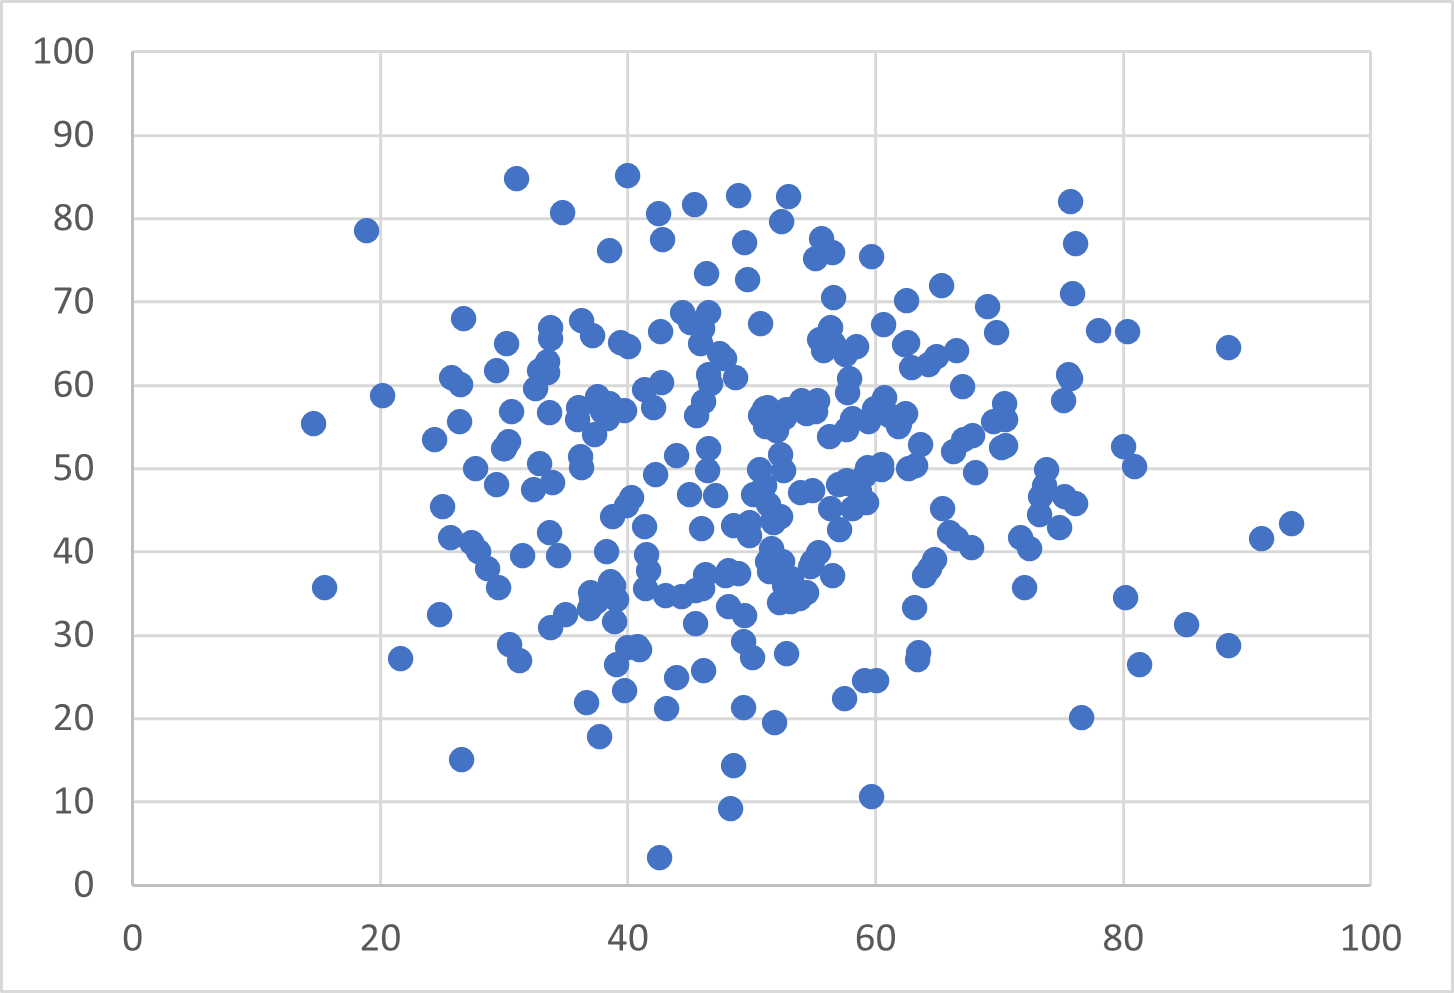
\includegraphics[width=0.3\textwidth]{Images/NormalScatter.png}
    \caption{Just some scattered data.}
    \label{fig:Scatter1}
\end{figure}

\subsubsection{Exercise}
Try adding the "Pie.png" image which is in the "Images" folder as a new figure. Note that all images you load must first be uploaded to the file system to the left of the page.

\subsection{Multiple Figures}
If you are comparing multiple figures, it might be helpful to embed them into a single figure as subfigures as we can see in figure \ref{fig:twoFigs}.

\begin{figure}[ht]
     \centering
     \begin{subfigure}[b]{0.45\textwidth}
         \centering
         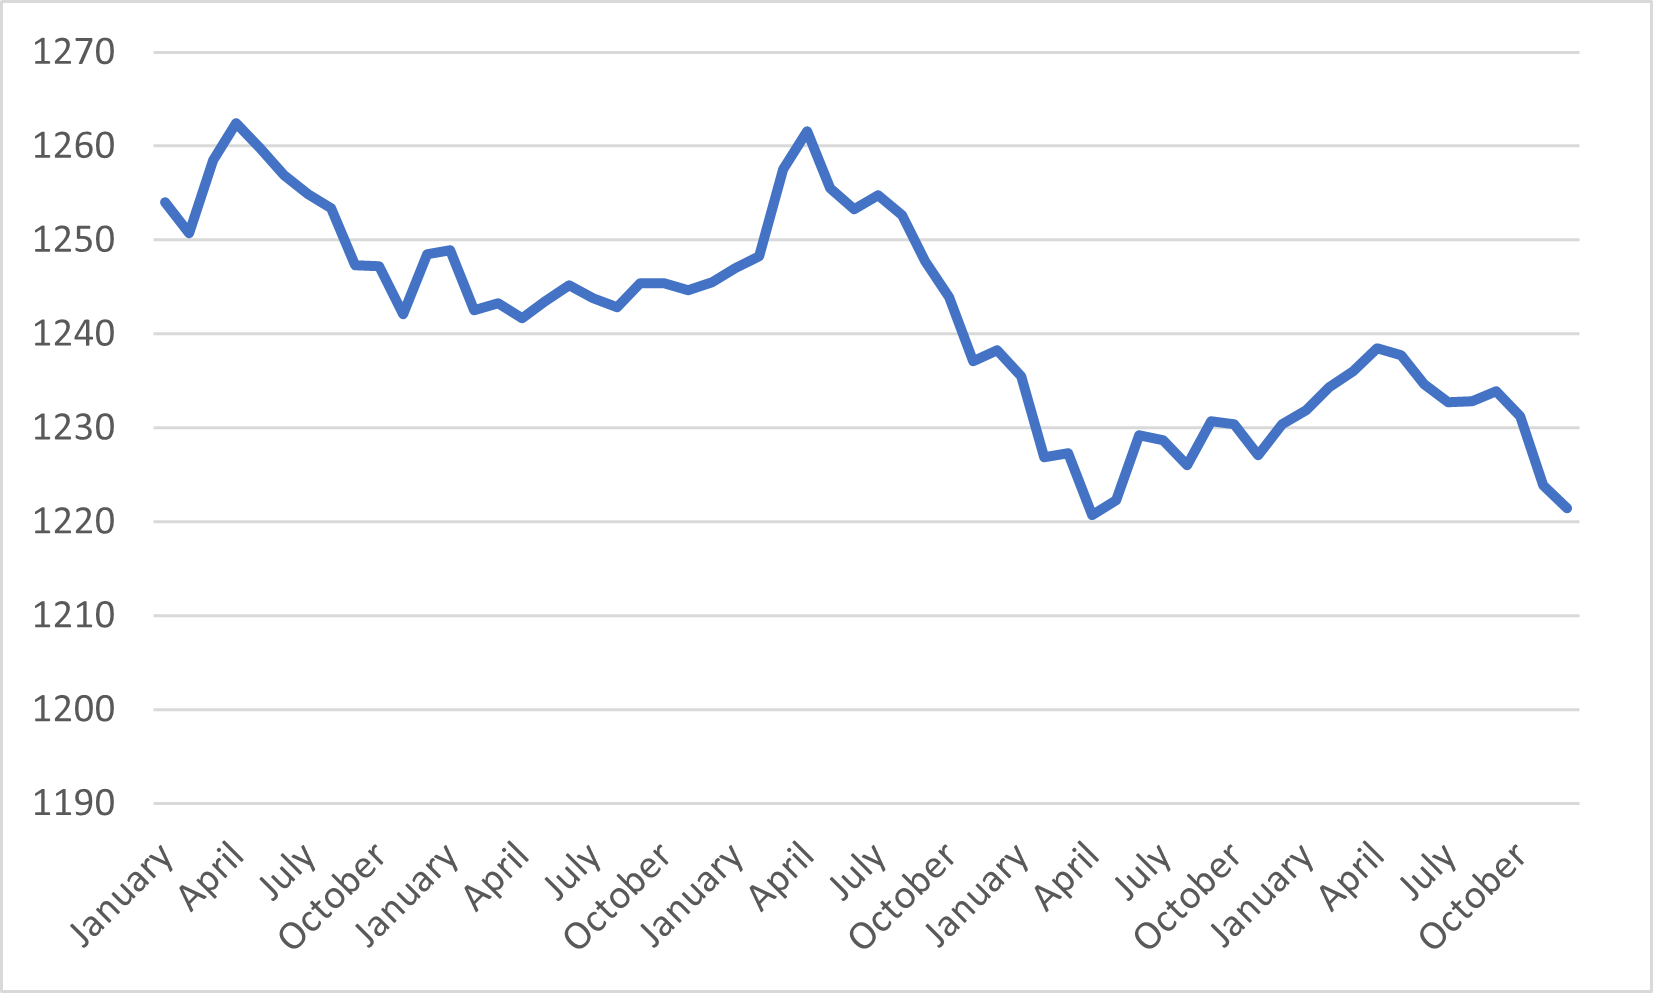
\includegraphics[width=\textwidth]{Images/TimeSeries.png}
         \caption{A time series of some stock.}
         \label{fig:timeSeries}
     \end{subfigure}
     \hfill
     \begin{subfigure}[b]{0.45\textwidth}
         \centering
         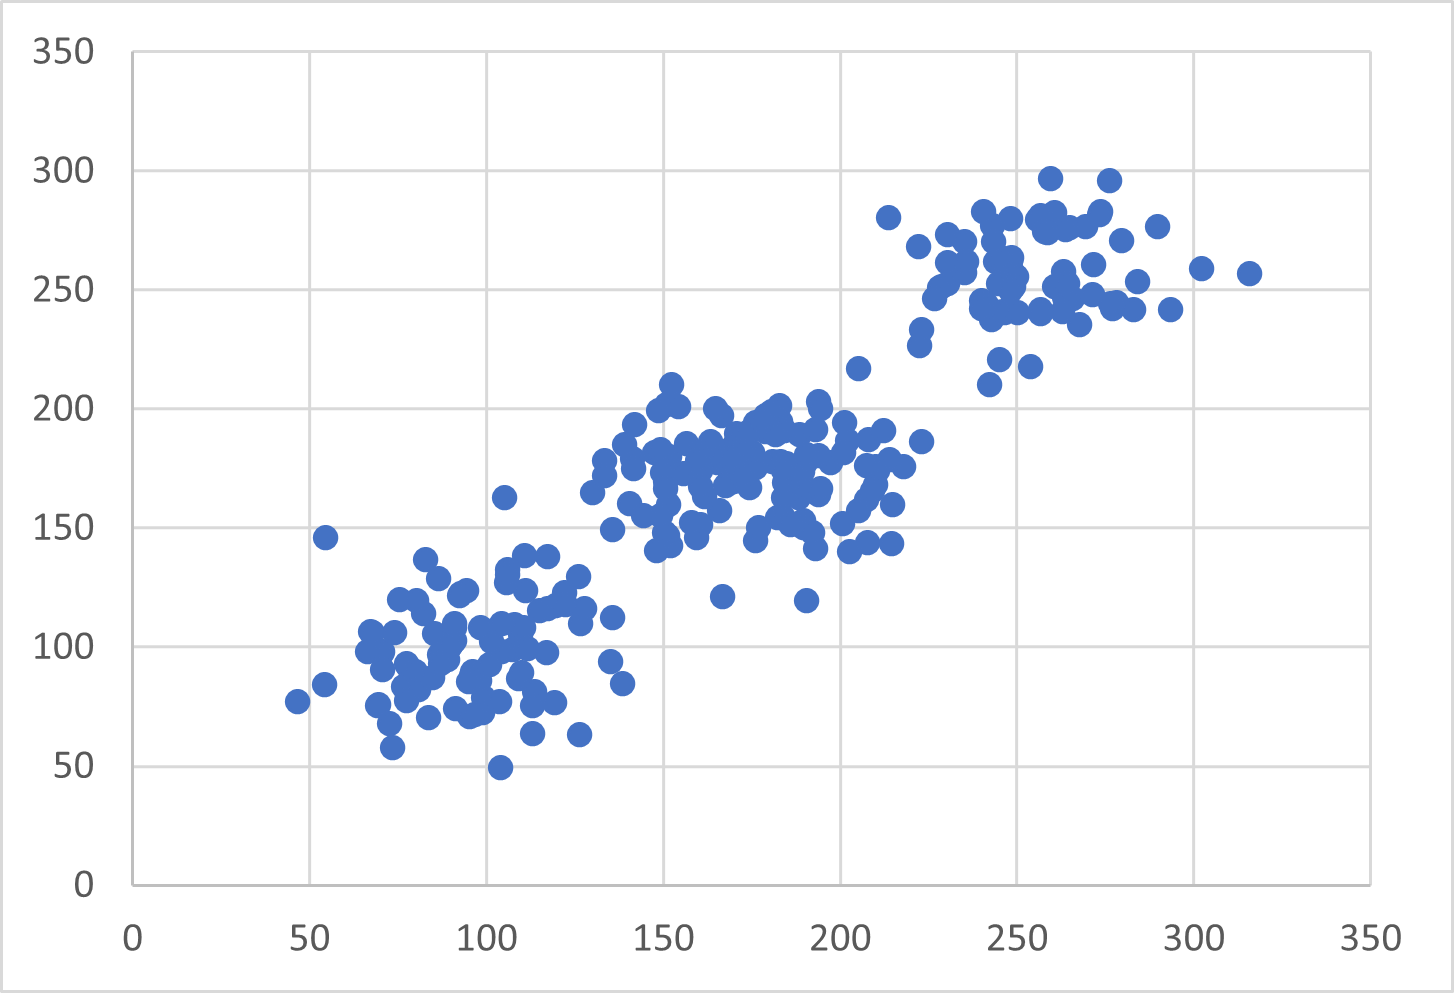
\includegraphics[width=\textwidth]{Images/Clusters.png}
         \caption{A scatter plot showing some clustering.}
         \label{fig:clusters}
     \end{subfigure}
        \caption{Two figures.}
        \label{fig:twoFigs}
\end{figure}

\subsubsection{Exercise}
You can embed many subfigures into a single figure, but make sure you alter the figure width and use the \verb|\hfill| commands to make the figure look neat!
For this exercise, find some images on the internet, upload them to your file system and try making a figure with 3 or more subfigures.


\section{Citation examples}
When writing academic reports it is very important to use citations to correctly credit other authors. Note that any quotes, images or ideas that you utilise in your work without a reference is \textbf{plagiarism} and will be punished.
However, the nature of coursework for this module means that references are not strictly required, and you should be able to gain top marks without any citations, but if you feel that your work would be improved by referencing another source you are free to do so, and should then include the correct citations and a bibliography.
Regardless, using citations in \LaTeX is one of it's great strengths, so I have left in a small section going over the basics.
In our school (especially for the final year project), it is recommended to adopt the Harvard style as a citation style. 
The followings are examples of citations using the Harvard style given in \href{https://www.overleaf.com/latex/examples/a-simple-example-showing-how-to-create-harvard-style-referencing-in-latex/mnwzgkyvdbyy}{A simple example showing how to create Harvard style referencing in LaTeX}.
Wherever students cite some papers to reinforce their description, they shall summarise the discussion in the paper correctly.  
The following is examples of citations\footnote{these are examples given in \url{https://www.overleaf.com/latex/examples/a-simple-example-showing-how-to-create-harvard-style-referencing-in-latex/mnwzgkyvdbyy}}.
\begin{enumerate}
\item A citation command in parentheses \parencite{Smith:2012qr}: \verb|\parencite| command \parencite{Smith:2012qr}.
\item A citation command for use in the flow of text: \verb|\textcite| command: As \textcite{Smith:2013jd} said \dots
\end{enumerate}

These citations is realized by BiBLaTeX commands. A quick cheat sheet for BibLaTeX commands is available in \href{http://tug.ctan.org/info/biblatex-cheatsheet/biblatex-cheatsheet.pdf}{Biblatex Cheat Sheet}.

\subsection{Exercise (Citation) 1}
Try citing ``Neocognitron: A hierarchical neural network capable of visual pattern recognition'' authored by Kunihiko Fukushima using Google Scholar to obtain the BibTex information. 

\subsection{Exercise (Citation) 2}
Try citing ``Very deep convolutional networks for large-scale image recognition'' authored by Simonyan and Zisserman using Google Scholar to obtain the BibTex information.

\section{Conclusion}
I hope this introduction to \LaTeX has been helpful for you, however this document really is just scratching the surface of what you can do with the software 
The best way to learn is to start writing documents in \LaTeX and seeing what problems you encounter and what solutions are suggested on the internet, as there is now a large community of people who use \LaTeX for their word processing every day, with there being a plethora of writing guides and forums where every problem you can think of has (probably) been answered.
If you want to learn more I would recommend going through the page \href{https://www.overleaf.com/learn/latex/Learn_LaTeX_in_30_minutes}{Learn Latex in 30 Minutes} on Overleaf to introduce you to even more functionality.


% This command will create a reference list for you. In the coursework I am going to set a reference list is not mandatory, but if appropriate you may want to include one, but being able to reference properly in \LaTeX is a useful skill to have!
\printbibliography


\end{document}
